% This file is iccc.tex.  It contains the formatting instructions for and acts as a template for submissions to ICCC.  It borrows liberally from the AAAI and IJCAI formats and instructions.  It uses the files iccc.sty, iccc.bst and iccc.bib, the first two of which also borrow liberally from the same sources.


\documentclass[letterpaper]{article}
\usepackage{iccc}

\usepackage[utf8]{inputenc} % Required for inputting international characters
\usepackage[T1]{fontenc} % Output font encoding for international characters
\usepackage{times}
\usepackage{helvet}
\usepackage{courier}
\usepackage{pgfplots}
\usepackage{tabu}
\usepackage{csquotes}
\usepackage{booktabs}

\pdfinfo{
/Title (an evaluation of the impact of constraints on the perceived creativity of narrative generating software)
/Subject (Proceedings of ICCC '18)
/Author (Lewis Mckeown)}
% The file iccc.sty is the style file for ICCC proceedings.
%
\title{An Evaluation of the Impact of Constraints on the Perceived Creativity of Narrative Generating Software}

\author{Lewis Mckeown\\
School of Computing\\
University of Kent\\
Canterbury\\
lam54@kentforlife.net\\ 
\And Dr. Anna Jordanous\\
School of Computing\\
University of Kent\\
Medway\\
a.k.jordanous@kent.ac.uk\\
}
\begin{document} 
\maketitle

\begin{abstract}
\begin{quote}
%There are a variety of ways to understand the computational generation of narratives. This paper considers them along a spectrum which arises from the application of constraint. This provides the groundwork for an investigation into the impact of constraints on the perceived creativity of the output of narrative generating systems. This supports the assessment of narrative generation software in terms of a spectrum of constraint application.
This work attempts to understand what level of constraint application results in the most creative output, by investigating the impact of constraints on the perceived creativity of the output of narrative generating systems. To achieve this, software is written that generates short stories, using adjustable levels of constraint meant to reflect those utilised by other narrative generating systems. These systems are presented at different positions along a spectrum, which we posit arises from the application of constraint. The creativity of the output is then assessed by human evaluators. The results are promising and show a clear variation of response based on the level of constraint imposed on the narrative generation process. The results show a sweet spot for maximal creativity closer to the less constrained end of the spectrum, which demonstrates the potential for more creative software by the relaxing of constraints. \end{quote}
\end{abstract}

%----------------------------------------------------------------------------------------
%	INTRODUCTION
%----------------------------------------------------------------------------------------
\section{Introduction}
%%Contributions of the paper%%
	%What it's trying to achieve and why
	%-Work Sharples quote about constraints in? 
Traditionally narrative generation systems have focused on generating outputs that can be proven to adhere to a particular narrative theory \cite{Perez2015}  or that greatly restrict the scope of what is possible \cite{leon2008creative} to ensure what is sometimes referred to as appropriateness \cite{Sharples96anaccount}. This project removes some of the first order assumptions about what constitutes a coherent narrative in an attempt to see if these constraints are in fact a hinderance to the creative potential of software.\\ 
\\By adjusting constraints that are often taken for granted when developing a narrative generation system, their impact can be assessed and the extent to which they may or may not affect the attainment of transformational creativity as defined by Boden \cite{BODEN1998347} can be measured. By doing so this work investigates whether a more relaxed narrative generation system might produce works that are perceived to be more creative. These adjustments tread a fine line, as too relaxed or too moderate applications of constraint will result in much lower creativity ratings. If a system strays too close to randomness, the perceived creativity will be heavily penalised. In contrast our results showed that the strictest application of constraints demonstrated the second highest level of creativity when evaluated by humans.\\
%Re-write once the focus has shifted towards the research question and results!
\\In the following sections a selection of existing systems are presented and shown to represent a spectrum of constraint application. How this spectrum motivates the choice of evaluative methods is then discussed, followed by an introduction to the software that was written to test the impact of constraints and the data gathering methods, finally a detailed discussion of the findings is presented.

%----------------------------------------------------------------------------------------
%	Anna's section about general constraints
%----------------------------------------------------------------------------------------
%Put Anna's section in with some goals and achievements - 

%----------------------------------------------------------------------------------------
%	The spectrum of constraints
%----------------------------------------------------------------------------------------
%Include paragraph from chapter 2 of dissertation? 
	%Software which creates artefacts that demonstrate true creativity, particularly within the domain of narrative generation, must then, fall somewhere between these two extremes of the spectrum. Without placing too high a stock in constraints that must be adhered to or narrative theory that must be replicated. Whilst still not leaving many traditional narrative concepts in the dust and combining letters in the hopes of generating a great work.
\section{The Spectrum of Constraint Application in Narrative Generating Software} \label{sec:spectrum}
The software discussed in this Section spans a range starting with context aware and goal oriented systems, which can themselves vary significantly in their application of constraint, to writing systems at what might be considered the other end of this spectrum; in which no character or context awareness could reasonably said to be present, but a large corpus of existing texts forms the knowledge base from which the software learns and generates new artefacts.\\
\\Carlos Le\'on and Pablo Gerv\'as made the storytelling system CAST to generate narratives based on the exploration and transformation of constraint rules \cite{leon2008creative}. CAST starts with a knowledge base of facts and a set of constraints on how those facts can be combined. It then works to combine the facts in a way that is considered coherent given the constraints in place. This might involve considering a sequence of actions like\\
\begin{equation}
kill(criminal, policeman) \rightarrow eat(policeman, sandwich) 
\end{equation}
as invalid, as the dead policeman can not eat a sandwich. \\
\\Simply combining facts however will not lead to satisfying or creative output, it could at best achieve Boden's combinational creativity in a naive sense. The authors acknowledge this and attempt to circumvent it by ensuring the knowledge base evolves with each combination of ideas. They even go so far as to say that allowing a small number of non valid states to be used can lead to an increase in creativity. A point that is not touched on much, but hints at Sharples' insistence that breaking constraints will likely enhance creativity \cite{Sharples96anaccount}. However Sharples also stated that the application of constraint is necessary, to ensure that what is generated does not become \enquote{a ramble of nonsense} this fact appears to have influenced the authors more as they are keen to avoid the generation of narratives that might be considered partial or non coherent \cite{leon2008creative}. Perhaps imposing a constraint on the system that might limit the potential for radical originality or the development of new aesthetic modalities.\\
\\P\'erez y P\'erez's system MEXICA \cite{Perez2015} generates stories about the inhabitants of ancient Mexico City using the engagement, reflection model  of narrative generation discussed by Sharples \cite{Sharples96anaccount}. This model involves a process of generation called engagement, in which MEXICA combines contexts from its knowledge base, looking for similar contexts to put together. This is followed by a process of reflecting and criticising the work developed so far, checking that preconditions can be satisfied and attempting to evaluate novelty. The goal is to guide generation as it happens and avoid creating narratives that are too similar to existing stories in the agent's knowledge base or stories which do not adhere sufficiently to the Aristotelian narrative structure, thus ensuring novelty and creativeness \cite{Perez2015,PEREZYPEREZ200415}. However given the imposition of an established narrative structure that must be maintained, and the avoidance of certain factors such as repetition or similarity, even though a certain amount of adaptability is inherent in the engagement reflection model, it is still very constrained in the amount of transformation or exploration that will be permitted.\\
\\Mueller and Dyer in their software DAYDREAMER explore the utility of daydreaming in machines, attempting to provide a computer model for daydreaming that will generate short stories that benefit from the imagination and creativity present in many daydreams \cite{Mueller1985}.\\
\\DAYDREAMER utilises a relaxed planning mechanism to guide the actions of a daydreaming agent. Mueller and Dyer posit that the relaxed set of constraints imposed on the daydreaming mind can facilitate the exploration of possibilities that would not normally have been pursued which can in turn allow for the exploration of unusual or not often linked ideas within the conceptual space. This relaxed approach to narrative can lead to \enquote{fortuitous analogy recognition}, creating a new or unusual idea which can be used to further enhance existing ones or progress a narrative towards resolution (\citeauthor{Mueller1985}  \citeyear{Mueller1985} P.3). This application of constraints in narrative generation increases the potential for radical originality if the conceptual space is made more flexible.\\ 
\\Mueller writes that
\begin{quote}
There are certain needless limitations of most present-day artificial intelligence programs which make creativity difficult or impossible: They are unable to consider bizarre possibilities and they are unable to exploit accidents.\\
(\citeauthor{Mueller:1990:DHM:77492} \citeyear{Mueller:1990:DHM:77492} P.14)
\end{quote}
This is a rather novel approach in the domain of narrative generating systems, which often focus on the adherence to an established narrative structure or literary theory. Actively seeking the bizarre or the accidental discovery of new combinations or transformations of ideas seems far more likely to generate creative works. To achieve this there must be some level of constraint to ensure appropriateness but the extent to which other aesthetic or structural facets of narrative are required is greatly reduced by DAYDREAMER.\\
\\There are still, however, defined goals involved that the daydreaming agent works towards and there is little discussion of adjusting the constraints imposed by the relaxed planning mechanism. So the narrative development still happens within a context aware system, progressing the goals of an agent to create a narrative. This is a constraint that few creative systems that produce a narrative seem willing to break.\\
\\Benjamin \cite{githubUniverseTalk} is a long short-term memory recurrent neural network that has developed several screenplays, like Sunspring \cite{SunspringScreenplay}. Unlike the other systems discussed, Benjamin works without agents trying to achieve goals, or sets of facts that ensure consistency when manipulating data from its knowledge base. Using a large corpus of existing screenplays it can be trained to learn and develop its own narratives in a style learned from the corpus provided \cite{githubUniverseTalk}. This is an application of deep learning that has been applied before in creating artistic works with an aim of learning and maintaining a structure\footnote{An LSTM RNN has been used to learn and compose its own blues licks with a particular focus on structure \cite{Eck2002}.} and which shows potential as a more modern avenue for creative software.\\
\\Developing story telling software that is not explicitly tasked with creating characters and managing their interactions is quite far removed from other narrative generating software discussed up to this point and its results are vastly different. They certainly would not be highly rated by P\'erez y P\'erez's implementation of the three layers model (discussed in the next section) and would likely be considered incoherent by the standards of CAST. However without the level of constraint implicit in the requirements for characters with predetermined goals, Benjamin's output could have the potential for far more unusual or bizarre ideas. There is the ability to exploit accidents, though perhaps not in the way intended by DAYDREAMER's authors, but the combinations of ideas present in works of this type are still, exactly that, present. The model and the steps used to arrive at the output may be more opaque than in the other systems, and it is harder for the system's knowledge base (excluding the corpus provided for inspiration) to be presented in a human readable way but the results and methods could be considered closer to a truly generative act than other more structured or constrained systems. The curation coefficient of the programmers is less obvious and the results will likely provide more of the \emph{shock} of surprise Boden anticipates when seeing something truly creative \cite{BODEN1998347}, as even knowing the corpus provided, the resultant artefacts are unlikely to be something the programmers would have predicted.\\
%Too weird/unstructured
% Character arcs and consistency is valued structure and similarity to an established canon is not necessarily ideal
% Closer to a truly generative act, arguably less of a curation coefficient than the other systems. 
\\The variety of responses from artistic works made by neural networks definitely shows the potential for an AI system developing an aesthetic modality that is distinct from that of humans, and it is arguably transforming the conceptual space with its abstract approach to generating text. However, Benjamin's works are the most likely of the systems discussed so far to be accused of becoming a \enquote{ramble of nonsense} by Sharples. This could perhaps be countered with a discussion of the audience and creative aspects systems like Benjamin are trying to attract and replicate. However given the variation from the corpus, it is clear that there may be more than a different aesthetic taste separating Sunspring from A New Hope.\\
\\There is undoubtedly time for art like this to establish itself and maybe even provide Boden's vindication of AI creativity, but it seems that right now some constraint in the form of context awareness may help improve the public opinion of this esoteric approach to narrative generation. This motivated the search for an application of constraint which would illicit the highest rating of creativity from audiences, when compared to other positions on the spectrum.
%----------------------------------------------------------------------------------------
%	Evaluation Models
%----------------------------------------------------------------------------------------
\section{Evaluating Computational Creativity in Narrative Generating Software} \label{sec:eval}
The following Section covers two methods for evaluating the creativity of narrative generation systems and compares their potential utility with regards to assessing the impact of constraints on creativity as well as assessing creativity in general. The aim is to highlight how  some methods of evaluation may be biased in favour of systems towards the more constrained end of the spectrum. As many evaluation techniques focus on an adherence to a structure or use other criteria that would be unfavourable methods of assessment given the foundational assumptions this paper aims to challenge. 
\\
% Three layers
\\P\'erez y P\'erez developed the \emph{Three Layers} approach to evaluating computer generated narratives to give the MEXICA plot generator the ability to assess its own output and the output of other writers. The model generates a score for the plot that can be used to quantitatively assess its potential creativity \cite{y2014three}.\\
\\Layer 0 of the model involves checking for required-characteristics  which are fundamental for something to be considered as having a plot. This layer does not contribute to the overall score, but a failure to meet the requirements of the model (due to unfulfilled preconditions or similarity to existing stories), will result in no evaluation taking place as the next two layers will not be completed. Layer 1 assesses the core characteristics of a narrative. Checking for the presence of climax, closure and unique or novel structures. The final layer deals with what P\'erez y P\'erez calls \emph{enhancers} and \emph{debasers} and it looks for aspects of narrative structure that if missing would be noticed immediately as their presence is taken for granted, P\'erez y P\'erez calls these preconditions and their absence is  penalised \cite{y2014three}. Repeated sequences are also penalised and reintroducing complications is considered an enhancer. Once the narrative has been evaluated by all layers of the model a score can be provided for each layer based on the presence or absence of these valued features and the way they are structured.\\
\\This method is not without its flaws, the most glaring of which is that the idea of automating the quantitative assessment of the creative worth of an artefact is highly suspect. The model requires a level of human curation in the selection of required characteristics for layer 0 and layer 1 focuses on the inclusion of core characteristics like climax chosen by the author. P\'erez y P\'erez says that \enquote{a narrative without climax is not a story} (\citeauthor{y2014three} \citeyear{y2014three} P.5); a highly subjective statement that relies on aesthetic taste rather than some quantitative measure of worth. It almost appears that in an attempt to remove the human component from the evaluation of works, the imposition of one humans judgements has been automated. This is a level of subjectivity that although not the direct definition appears to be an example of too high a curation coefficient. Although the layers of the model can be tweaked, as acknowledged by the authors, the same issue will likely remain, that the criteria will be chosen by one or a small group of people and are relatively inflexible once in place. This model might be seen as imposing constraints in a way that penalises variation from expected norms, in light of this it is unlikely to value the transformation of the conceptual space in a way that might result in unusual or new aesthetic measures that truly great creative works can facilitate. The problem of self evaluation is covered by Boden who stated that it would be harder to solve than the generation of works by AI \cite{BODEN1998347}.\\
\\Rather than try and skirt the need for human subjectivity in the evaluation of creativity then, it might be better to embrace it. In an earlier paper P\'erez y P\'erez and Sharples wrote some criteria for presenting narrative software for evaluation. They highlight that a common difficulty when assessing story generation systems is the lack of an agreed upon comparative structure \cite{PEREZYPEREZ200415}. To solve this they proposed some rules for evaluation stating that
\begin{itemize}
\item The programs knowledge base should be available for human evaluation in a sensible form.
\item The type or aspects of creativity being modelled should be stated clearly by the designers, as should the audience.
\item The program should be capable of generating a minimum of ten stories, 3 of which can be selected by the designers for human evaluation.
\item The selected outputs should be \enquote{judged for overall quality, originality and interestingness by independent raters} (\citeauthor{PEREZYPEREZ200415} \citeyear{PEREZYPEREZ200415} P.15). The evaluators may or may not know that the stories were written by a computer.
\end{itemize}
This model is less programatic and perhaps harder to implement than the three layers. However it allows for a range of creative opinions to be included in the evaluation of the works by having multiple individuals assess them rather than implementing the automated checking of criteria. The less prescriptive approach can also be considered an advantage when viewed in this light too. As it may appear prima facie to be less quantitative to have output judged for originality, novelty or interestingness by humans; quantifying these ratings over a group of people is possible and their individual approaches to creative assessment could even be documented alongside their responses to provide further context to each evaluation.\\
\\When evaluating the output of creative narrative generating software, the use of human participants may not be ideal for uniform data gathering,  but it may represent the state of the art when assessing the novelty or creativity present in a work of art.\\

%----------------------------------------------------------------------------------------
%	SOFTWARE
%----------------------------------------------------------------------------------------
\section{The Software}
To support the investigation into the significance of constraints on narrative generation, some story writing software was developed. 
It was designed to produce narratives with a dark and dreamlike theme, taking inspiration from authors and creators like David Lynch, David Foster Wallace and Haruki Murakami among others. The goal was for the stories to replicate some of the style of magic realist or surrealist authors and auteurs, who demonstrate a high level of creativity whilst seeming to balk at the traditional constraints of narrative theory. \\

%\section{Initial Planning}
Early versions of the project considered using a combination self evaluation and human evaluation to assess the creative worth of generated stories. The output was to be generated by software that was using a relaxed ruleset that would be some combination of the algorithms and approaches commonly found in machine learning applications and the context aware, agent driven models such as DAYDREAMER and MEXICA. The original aim was to model the less constrained end of the spectrum, working under the assumption that a less restricted narrative generation system would be able to demonstrate creativity closer to that of the artists that inspired the project. Self evaluation was abandoned in favour of structured human evaluation and the project became more directed once the research question was narrowed, to focus on the impact of constraints in particular.\\

%\section{Evaluation Strategies and Constraint Application}
Once the decision was made to focus on constraints the evaluation strategy and implementation became key areas of focus. Initially the software's output was to be evaluated via comparison alongside other story writers which used differing levels of constraints such as CAST or DAYDREAMER. However due to the variety in style, length and availability of the other software's output it quickly became clear this was an unfit method of evaluation.\\
\\To establish a more rigorous way of evaluating the output, the decision was made that it all come from the same creative agent. The software would use the same knowledge base of characters and actions to generate narratives but do so with differing levels of constraint in place. Rather than using a relaxed ruleset that was a fixed set of constraints representing some position on the spectrum of creative writing software, these constraints should be adjustable by the user. The software's output could then be evaluated by humans with a version of P\'erez y P\'erez and Shaples' 2004 testing methodology.\\
\\The final version of the software allowed the algorithms that dictated, character actions, locations and events to be selected prior to generation, along with other critical aspects such as whether character death would remove them from the narrative or if duplicate characters could appear. This facilitated the generation of a selection of stories which could represent positions on the hypothesised spectrum of constraint allowing human evaluation to be carried out and the assessment of the significance of constraint on narrative generation to be performed.

%----------------------------------------------------------------------------------------
%	Evaluation Strategy
%----------------------------------------------------------------------------------------
\section{Evaluation Strategy}
To evaluate the output of the software a selection of P\'erez y P\'erez and Sharples' 2004 benchmarks for assessing story generation systems were used to develop an evaluation strategy based on user feedback strategy.\\
\\The benchmarks recommend stating the aspects or style of creativity that the software is attempting to model, as well as the audience it is aimed at. They also recommend that the software be capable of generating at least 10 stories, and that 3 of these could be selected by the software authors for human evaluation.\\ 
\\This model was adhered to very closely, with the final evaluation strategy involving 10 narratives being generated and 3 selected for evaluation. This process was repeated for 4 differing levels of constraints, for a total of 12 stories which required evaluation. Before being presented with the stories, an explanation of the project and its creative aims and target audience was provided to the respondent. This was presented alongside two dictionary definitions of creativity focused on the production of artefacts demonstrating unusual or non traditional ideas which served as a guide when answering to what extent the user believed each story demonstrated creativity, using the following scale
\begin{description}
\item[Strongly Agree:] 2
\item[Agree:] 1
\item[Neutral:] 0
\item[Disagree:] -1
\item[Strongly Disagree:] -2
\end{description} 
The respondents were also asked to indicate if they liked each story, This was primarily to separate opinions about whether creativity was being demonstrated from any other value judgements about the quality of the text.
% Perhaps more explanation on the creativity being modelled ?
\subsection{Creating the Datasets}
The options chosen to generate the datasets were developed to try and reflect a section of the spectrum of constraints used when generating narratives with software. The breakdown can be seen in Table \ref{table:datasets}.\\ 
% Include table?
\begin{table*}[h!]
\begin{tabu} {X[c] | X[c] X[c] X[c] X[c] X[c]}
\toprule
Datasets & Action Choice & Event Choice & Location Choice & Respect Death & Allow Doppelgangers \\
\midrule
Unconstrained & Random & Random & Random & False & True\\ \midrule
Moderately Constrained (Set 1) & Markov & Random & Random & True & False\\ \midrule
Moderately Constrained (Set 2) & Markov & Markov & Random & True & False\\ \midrule
Tightly Constrained & Character Motivation & Markov & Markov & True & False\\
\bottomrule
\end{tabu}
\caption[Breakdown of Datasets]{Breakdown of the options used to create each dataset for user evaluation.}
\label{table:datasets}
\centering
\end{table*}
%%
\\The lowest level, dubbed \emph{unconstrained}, was chosen mostly based on randomness, to represent the least amount of constraint a narrative could be generated with, this was meant to mimic an amount of context awareness at the level of an untrained neural network, and given the software's design, the curation coefficient likely played a large part in the resultant narratives, rather than an application of what might be deemed computational creativity by P\'erez y P\'erez's definition; \emph{c-creativity} which requires the generation of new and relevant knowledge \cite{PEREZYPEREZ200415}.\\
\\The other end of this spectrum was as \emph{tightly constrained} as the software could be, with actions chosen by character motivation, a Markov model used to select events and locations and the options to respect character death and prevent doppelgangers being imposed.\\ 
\\The two middle datasets represented as \emph{moderately constrained} were generated with a very similar set of options, the key difference being the choice in \emph{set 1} to select events randomly rather than using a Markov model, making it slightly less constrained than \emph{set 2}. Event choice and ordering is a non trivial aspect of any narrative and this could provide a significant impact on the resulting output. The aim was to represent more middling levels of the spectrum, with \emph{set 1} hopefully mimicking DAYDREAMER's less constrained and more esoteric approach to event choice, whilst still imposing a constraint over action choice. As a differentiator \emph{set 2} imposed a slightly stricter logic, perhaps more reminiscent of CAST's pursuit of coherence. Although the artistic style, approach to generation and undoubtedly, the output of each dataset was different to all of the systems used as inspiration; this should present an abstracted and high level representation of how constraints used in story writing systems can affect their output. The extent to which this is the case is discussed in the next Section.

\subsection{Getting Respondents}
Initial evaluations were completed by a small set of people who provided more detailed feedback and discussion following the completed assessment. Once these evaluations were completed, a post was made on the Computational Creativity Google group asking for respondents. This provided more discussion of the work and feedback gathering approach as well as a host of new respondents, 10 more complete responses in total. 
%A discussion of the results can be found in TKTK.

%----------------------------------------------------------------------------------------
%	ANALYSIS OF RESPONSES
%----------------------------------------------------------------------------------------
\section{Analysis of Responses}
A total of 202 evaluations were received during a one week run of feedback gathering, resulting in an estimated 16 respondents. Not all respondents completed the entire survey however, so some outliers were left that needed to be removed. 
Despite the presence of incomplete responses a trend developed early on and remained rather consistent throughout the evaluation process. The datasets representing \emph{tightly constrained} and \emph{moderately constrained set 1} were consistently deemed more creative than \emph{moderately constrained set 2} or the \emph{unconstrained} set. This trend continued, with some minor fluctuation; \emph{moderately constrained set 2} and \emph{unconstrained} jumped between being deemed uncreative and simply neutral,  ultimately ending up with \emph{unconstrained} being evaluated as slightly less creative (see Figure \ref{fig:acr}). 

\subsection{The Impact of Constraints on Perceived Creativity}
The relative unsuccessfulness of the most aleatory dataset, \emph{unconstrained}, shows that Sharples' insistence on appropriateness and its pursuit by software representing the more constrained end of the spectrum such as CAST and MEXICA is thoroughly justified. Even given the type of creative endeavour that the project was attempting to emulate - surrealist and magic realist authors, known for bizarre juxtaposition in their work - the outputs generated using only random combinations of story components were consistently deemed less creative and liked less than their more constrained counterparts.\\ 
\\The \emph{tightly constrained} dataset, the end of the spectrum in which every thing that could prohibit randomness was in place, showed the second highest level of creativity according to respondents and was liked the most. The potential for more clear character arcs, as this was the only dataset using character motivation, may help identify its popularity. One respondent in more detailed feedback even correctly identified a story from this dataset as showing evidence of character motivation. This might lead to an audience seeing more familiar tropes such as revenge or love and associating the output with works they have a clear mental model for and enjoy. The issue of conflating a positive response to the work with the presence of creativity is discussed in the next Section.\\
\\The most interesting results came from the juxtaposition of the two middle datasets. With \emph{moderately constrained set 1} rating the most creative of all four datasets, whereas \emph{set 2} was consistently among the lowest creativity ratings, \footnote{With outliers removed, this was revealed to be the fault of one story significantly affecting the (low) average. See co880.lewismckeown.com.} scoring just higher than \emph{unconstrained} once the outliers were removed.\\
\\The only difference between the two middle datasets was the choice of event being made randomly by \emph{set 1} and by Markov model in \emph{set 2}. This distinction could represent a violation of constraint in the ideal sense that Sharples writes about, in a way that may facilitate radical originality whilst maintaining appropriateness.\\
\\Event choice is significant, however, the most constrained narrative generation systems focus primarily on the restriction of character action to ensure an arc or predictable response to stimuli. Beyond this, perhaps there is a lot of room for manoeuvre when developing what happens around characters. The potential for the bizarre with a less constrained selection of events and locations is greatly increased and may result in a potential transformation of the conceptual space, when juxtaposed with more considered character interactions. It would be charitable to attribute a level of Boden's transformational creativity to this project, but it should demonstrate the importance of a proper assessment of constraint to finding a computer model for transformational creativity.
%pgfplot ACR%
\begin{figure}[h!]
\centering
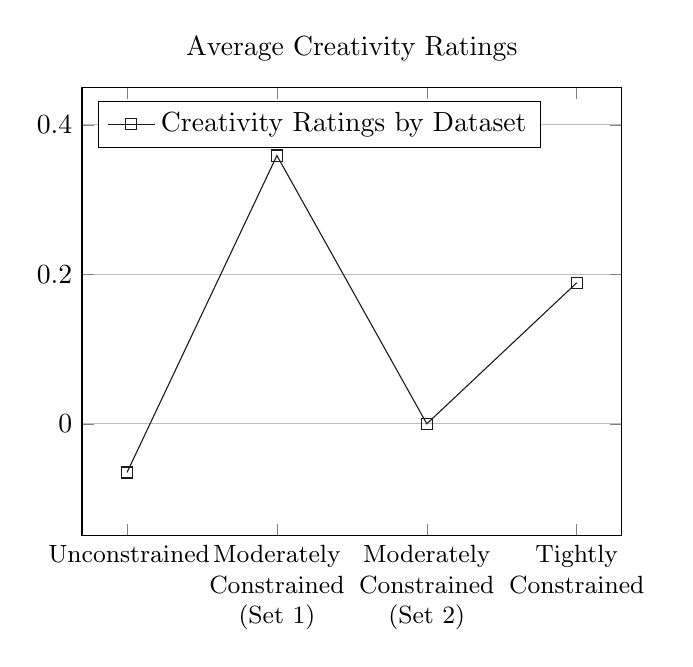
\begin{tikzpicture}
\selectcolormodel{gray}
\begin{axis}[
    title={Average Creativity Ratings},
    ymin=-0.15, ymax=0.45,
    xtick=data,
    xticklabels={Unconstrained,Moderately Constrained (Set 1),Moderately Constrained (Set 2), Tightly Constrained},
    x tick label style={font=\small,text width=2cm,align=center},
    legend pos=north west,
    ymajorgrids=true,
]
 
\addplot+[sharp plot][
    color=blue,
    mark=square,
    ]
    coordinates {
    (0,-0.0652)(1,0.359)(2,0)(3,0.1887)
    };
    \legend{Creativity Ratings by Dataset}
\end{axis}
\end{tikzpicture}
%\decoRule
\caption[Average Creativity by Dataset]{Average creativity ratings for each dataset.}
\label{fig:acr}
\end{figure}
%%
\subsection{Aesthetic Taste and Perceived Creativity} \label{sec:aesthetics}
In keeping with the thoughts of some respondents the extent to which people indicated they liked the story largely correlated with a positive creativity rating. With only 8 responses indicating that they liked a story that they considered not to be showing creativity and 16 responses indicating that they disliked a story that they agreed demonstrated creativity. This is opposed to the 64 responses indicating a story was liked and demonstrated creativity and the 49 indicating a story was not liked and did not demonstrate creativity.\\
\\The choice to ask how creative each story was separate from whether a respondent liked it was primarily to remove assessments of quality or personal preference from judgements about creative merit. However given the correlation between creativity ratings and respondents liking the story, it seems quite likely that the aesthetic tastes of the evaluator play a large role in their assessment of an artefact's creative worth. This has interesting implications for Colton and Wiggins, who indicate that a creative machine may have different aesthetic tastes to humans. It highlights the difficulty of machines being considered creative without first mimicking existing human aesthetic standards. To provide aesthetic measures with which to assess their work or a commentary on the motivations behind it then, as Colton and Wiggins suggest \cite{Colton_computationalcreativity}, may be a crucial step for creative machines to both achieve creative independence and be judged as having done so by human evaluators.

%----------------------------------------------------------------------------------------
%	SUMMARY AND EVALUATION
%----------------------------------------------------------------------------------------
\section{Summary of the Data}
Overall the stories were deemed more creative than not, and respondents liked and disliked them in almost equal measure. The ratio of stories which were liked to those that were disliked could be attributed to the niche narrative style and sources of data that the software used.\\
\\The higher presence of creative to not creative output is promising for the software and any future development it might undergo. It also demonstrates the rich creative potential that non traditional and surrealist works present to creative systems. This may reflect a similitude between human made surrealist art and AI generated works.\\ 
\\The results (shown in Figure \ref{fig:acr} and co880.lewismckeown.com), demonstrate that works without any effort to retain appropriateness as defined by Sharples \cite{Sharples96anaccount} will result in unfavourable creativity ratings, as seen by the response to the \emph{unconstrained} dataset. In contrast pursuing appropriateness, as the \emph{tightly constrained} set did, will demonstrably improve perceptions of creativity by human evaluators. This disproved an early hypothesis which assumed that less restriction imposed on the narrative generation process would result in higher creativity ratings for the resulting artefacts.\\ 
\\The most exciting finding, is that striking a balance between the pursuit of appropriateness and the breaking of constraint, will lead to far higher creativity ratings, hopefully demonstrating the significance of constraint application in any attempt to model transformational creativity as described by Boden \cite{BODEN1998347}.

\subsection{Evaluation of the Data}
The project was ultimately an investigation, so any feedback and data returned would constitute some form of success. The interesting conclusions that can be drawn from the data and the number of encouraging responses, however, made the investigation both satisfying and rewarding. Despite this there are several areas in which improvements could be made, particularly with regards to the testing methodology and feedback gathering.\\
\\Several users commented on the repetition present in the evaluated stories. They were generated from a knowledge base consisting of only 34 actions, 25 locations and 24 events. This could have been increased to reduce potential fatigue of the users, as it could affect their ratings, particularly later in the process. The story order could also have been randomised rather than fixed, although for individuals this would make no difference, for the results as a whole it might have reduced the chance of later stories being rated as less creative because of perceived repetition. Although given the creativity ratings seen in Figure \ref{fig:acr} it appears this did not happen, with a larger dataset it would have been prudent.\\
\\In some feedback the genre of stories was criticised for perhaps letting a less cohesive work be presented as a completed one.\footnote{It was suggested that this might be \enquote{sleight of hand} by one respondent. Hopefully this Section proves there was nothing up the authors sleeve.} However the project was intentionally developed in a way such that the subversions - for the most part - were intentionally done. There were toggles set when adjusting constraints before generating a story that would allow a character who had just died to have dinner with their murderer and a toggle that would allow two identical characters to go on a road trip. The intention being to knowingly subvert traditions and the expectations of readers (with an option to retain the more logical outcomes by adjusting the constraints) rather than to merely stumble into incoherence. The fact that randomly arriving at creativity is unlikely is also supported by the consistently low creativity ratings of the \emph{unconstrained} dataset and the higher ratings of the more tightly developed datasets. So, although this is an understandable criticism, it is hopefully addressed sufficiently here and in the preceding sections.\\
\\Another similar criticism received from users, was to what extent the output could be considered a story, or if it was insufficiently fleshed out to be one. The stories were presented as short vignettes before asking for evaluation, to prepare users for the format. The format was chosen to be as concise as possible to allow 12 stories to be read consecutively without fatiguing the reader and affecting subsequent ratings.\\
\\The form of the stories relates to a struggle later in the project between the fabula and the discourse. All the components were created and put in order as the software generated the narrative, but a selection of JSON objects is unlikely to be considered a story. So this later stage of the project struggled with the difficulty of attempting to reconcile the fabula generated into a discourse that could be presented in a way that humans could enjoy (or not). With more time and thought the presentation would have been adjusted and perhaps incorporated into the user feedback more comprehensively. However the stories were introduced as outlines to manage expectations. So although this was an element that could undoubtedly have been polished, for efficiency and user experience, shorter and more quickly digestible narratives seemed appropriate.

%----------------------------------------------------------------------------------------
%	FUTURE WORK
%----------------------------------------------------------------------------------------
\section{Future Work}
To a large extent the objectives set out in the introduction were met over the course of the project. However there are several areas in which the work could be developed further and potential alternate avenues of research that it could provide a foundation for.\\
\\An obvious continuation of the work could involve completing unfinished features such as inverting character motivations and allowing the mixing of components and consequences more freely. Although this would require some changes to the knowledge base it would increase the variability of the output and allow for more combinations to be made with fewer story components, also potentially increasing the likelihood for the unusual ideas and combinations that proved a fruitful creative source throughout the project.\\
\\If given more time, the project would also greatly benefit from the gathering of more user feedback. The feedback process could perhaps be refined and the story order randomised to reduce fatigue and potential bias. More feedback would help to see if the trends that started with a very small number of respondents hold over a larger group.\\
\\If the trends established by this project hold when a larger number of evaluations have been completed, it may be valuable to take a more fine grained approach to the research; perhaps investigating how constraints applied to one particular aspect of story such as action choice or character arc can affect the creativity of the resulting narratives.\\

%----------------------------------------------------------------------------------------
%	CONCLUSION
%----------------------------------------------------------------------------------------
\section{Conclusions and Key Findings}
When starting this project an early hypothesis was that the less constrained a narrative generation system was by rules or convention, the more potential for creativity was present. This hypothesis was proved wrong, with the least constrained narratives being consistently chosen to demonstrate less creativity than the more constrained ones. However a potential sweet spot was found with minimal constraint applied to every aspect of narrative generation modelled except for character actions. The results show the areas in which constraint application appears are critical, but also highlight the freedom in other areas to relax what might be considered necessary impositions on the narrative generating agent.\\
\\A secondary hypothesis was that the existing crop of narrative generating software could be presented as a spectrum of constraint application to the problem of generating narratives. This is well supported by the feedback gathered from user evaluations, which shows a clear variance of response to narratives generated with differing levels of constraint, in a manner that supports the reading of the literature presented in Section 2. This is further evidenced by respondents dislike for the more aleatory generation techniques and expressed preference for the more teleological with particular focus on character arcs.\\
\\Another key finding was that the aesthetic tastes of evaluators are closely related to their assessment of creativity. So for artificial models of creativity to produce outputs which differ widely from established human standards and still be considered creative, the work should be explained or justified in some way by the creative agent.\\
\\Overall the data gathered shows promise for further investigation into the impact of constraints that may often be taken for granted when writing and evaluating narrative generating software and how their removal or adjustment may lead to more creative AI. 

%\printbibliography[heading=bibintoc]
%\appendix{\LaTeX{} and Word Style Files}\label{stylefiles}

%The \LaTeX{} and Word style files are available on the ICCC-13
%website, {\tt http://computationalcreativity.net/iccc2013/}.
%These style files implement the formatting instructions in this
%document.

%The \LaTeX{} files are {\tt iccc.sty} and {\tt iccc.tex}, and
%the Bib\TeX{} files are {\tt iccc.bst} and {\tt iccc.bib}. The
%\LaTeX{} style file is for version 2e of \LaTeX{}, and the Bib\TeX{}
%style file is for version 0.99c of Bib\TeX{} ({\em not} version
%0.98i).

%The Microsoft Word style file consists of a single template file, {\tt
%iccc.dot}. 

%These Microsoft Word and \LaTeX{} files contain the source of the
%present document and may serve as a formatting sample.  

\bibliographystyle{iccc}
%\nocite{*}
\bibliography{CO880Bib.bib}

%\section{Temp Appendices}
%\begin{table}[h!]
%\caption[Average Creativity Rating of Stories]{Average creativity rating of stories, grouped by dataset, with 0 representing neutral, positive values being more creative and negative values corresponding to ratings indicating less creativity. This data is used to form the graph in Figure \ref{fig:acr}.}
%\label{table:cr}
%\centering
%\begin{tabu} {X[c]  X[c]  X[c]}
%\toprule
%Story ID & Dataset & Average Creativity Rating\\
%\midrule
%409 & Unconstrained & -0.1765 \\
%412 & Unconstrained & 0.0667\\
%416 & Unconstrained & -0.0714\\
%\midrule
%392 & ModeratelyConstrained1 & 0.3077 \\
%394 & ModeratelyConstrained1  & 0.5385\\
%399 & ModeratelyConstrained1  & 0.2308\\
%\midrule
%428 & ModeratelyConstrained2  & 0.0769\\
%430 & ModeratelyConstrained2 & -0.1538\\
%433 & ModeratelyConstrained2 & 0.0769\\
%\midrule
%422 & Tightly Constrained & -0.4211\\
%424 & Tightly Constrained & 0.5882\\
%425 & Tightly Constrained & 0.4706\\
%\bottomrule\\
%\end{tabu}
%\end{table}
%
%\begin{table}[h!]
%\caption[Breakdown of Datasets]{Breakdown of the options used to create each dataset for user evaluation.}
%\label{table:datasets}
%\centering
%\begin{tabu} {X[c] | X[c] X[c] X[c] X[c] X[c]}
%\toprule
%Datasets & Action Choice & Event Choice & Location Choice & Respect Death & Allow Doppelgangers \\
%\midrule
%Un-\newline constrained & Random & Random & Random & False & True\\ \midrule
%Moderately Constrained (Set 1) & Markov & Random & Random & True & False\\ \midrule
%Moderately Constrained (Set 2) & Markov & Markov & Random & True & False\\ \midrule
%Tightly Constrained & Character Motivation & Markov & Markov & True & False\\
%\bottomrule
%\end{tabu}
%\end{table}
%
%%pgfplot ratings totals
%\begin{figure}[h!]
%\centering
%\begin{tikzpicture}
%\selectcolormodel{gray}
%\begin{axis}[
%    title={Creativity Ratings (Totals)},
%    symbolic x coords={Creative,Not Creative,Neutral},
%   x tick label style={
%		/pgf/number format/1000 sep=},
%    ybar,
%    ymin=10, ymax=85,
%    grid=major,
%    xmajorgrids=false,
%    bar width=85pt,
%    xtick=data,
%    legend style={at={(0.5,-0.2)}, anchor=north},
%    enlarge x limits=0.25,
%    ]
%    \addplot coordinates {
%        (Creative,80)(Not Creative,57)(Neutral,40)
%    };
%\end{axis}
%\end{tikzpicture}
%%\decoRule
%\caption[Total Creativity Ratings]{Totals for each possible rating, creative, not creative or neutral.}
%\label{fig:crt}
%\end{figure}

%%Like to Dislike pgfplot
%\begin{figure}[h!]
%\centering
%\begin{tikzpicture}
%\selectcolormodel{gray}
%\begin{axis}[
%    title={Liked to Not Liked (Totals)},
%    symbolic x coords={Liked, Not Liked},
%    x tick label style={font=\small,text width=1.7cm,align=center},
%    ybar,
%    ymin=10, ymax=95,
%    grid=major,
%    xmajorgrids=false,
%    bar width=105pt,
%    xtick=data,
%    enlarge x limits=0.45
%    ]
%    \addplot coordinates {
%        (Liked, 89)(Not Liked, 88)
%    };
%\end{axis}
%\end{tikzpicture}
%%\decoRule
%\caption[Like to Dislike Ratio of Stories]{The total number of stories which respondents indicated they liked, set next to the total for which no like was indicated.}
%\label{fig:ltd}
%\end{figure}

\end{document}
